\documentclass[letterpaper, 10 pt, conference]{ieeeconf}

\IEEEoverridecommandlockouts
\overrideIEEEmargins

\usepackage[dvipsnames]{xcolor}
\usepackage{graphicx}
\usepackage{tikz}
\usepackage{etoolbox}
\usepackage{booktabs}
\usepackage{multirow}
\usepackage{amsmath}
\usepackage{verbatim}
\usepackage{colortbl}
\usepackage{amsfonts}
\usepackage{csquotes}
\usepackage{hyperref}
\usepackage{subfig}
\usepackage{placeins}
\usepackage{url}

\title{\LARGE \bf
AURA: Decentralized Deep Reinforcement Learning with Deterministic Safety Envelopes for Resilient Traffic Signal Control and Emergency Corridor Preemption
}

\author{Deepak R.$^{1}$%
\thanks{$^{1}$Department of Robotics and Automation, Dhaanish Ahmed College of Engineering, Chennai, India. Pre-print repository DOI: 10.5281/zenodo.20265628.}%
}

\raggedbottom

\begin{document}

\maketitle
\thispagestyle{empty}
\pagestyle{empty}

\begin{abstract}
Urban traffic signal optimization requires simultaneously addressing non-stationary civilian demand surges and life-critical emergency vehicle (EV) preemption. While Deep Reinforcement Learning (DRL) demonstrates superior adaptability over classical fixed-time schemes, existing learning-based methods frequently rely on unconstrained action spaces that risk phase starvation, lack deterministic physical safety guarantees, and cause severe post-preemption shockwaves in cross-street corridors. In this work, we propose \textbf{AURA} (\textit{Acoustic-visual Urban Routing Architecture}), a decentralized reinforcement learning framework that couples a Deep Q-Network (DQN) with a Deterministic Safety Envelope to optimize urban traffic throughput while guaranteeing safe phase transitions and resilient emergency corridor preemption. The safety envelope deterministically bounds green durations between 10\,s and 45\,s based on live queue lengths and strictly enforces mandatory 3-second yellow clearance intervals outside the learning policy. Furthermore, AURA integrates a rapid EV preemption mechanism and explicitly mitigates post-clearance queue accumulation. Evaluated within the microscopic traffic simulator Eclipse SUMO under Krauss car-following kinematics against three benchmark systems—Traditional Fixed-Time, Demand-Responsive Actuated control, and the theoretical Max-Pressure controller—across both controlled grid corridors and an authentic 183-intersection real-world OpenStreetMap network of Midtown Manhattan, AURA achieves remarkable performance. On the real Manhattan network, AURA slashes emergency vehicle clearance latency by 61.9\% (16\,s vs. 42\,s) and reduces average network halting queues to 26.33 vehicles (compared to 38.19 for Fixed-Time and 27.97 for Max-Pressure) while maintaining robust post-preemption shockwave recovery.
\end{abstract}

\section{Introduction}
\label{sec:introduction}

Urban traffic congestion represents an escalating challenge in metropolitan transportation management, directly correlating with economic inefficiencies, elevated greenhouse gas emissions, and life-threatening delays for emergency response vehicles (EVs)~\cite{webster1958, mnih2015human}. Conventional municipal intersections continue to rely predominantly on fixed-time or rule-based actuated signal controllers. While fixed-cycle timers are straightforward to implement, their inability to adapt to asymmetric flow rates leads to severe green starvation, where empty corridors are granted green allocations while congested lanes endure prolonged halts~\cite{lowrie1990scats}.

The limitations of traditional infrastructure become critically apparent during emergency vehicle routing. Ambulances, fire engines, and law enforcement units often face gridlocked intersection approaches. Existing preemption methods generally rely on either visual detection or acoustic siren triggers that force immediate all-red or green overrides~\cite{cucchiara2003detecting, salamon2014urbansound}. However, naively forcing preemption without modeling the surrounding traffic dynamics frequently causes severe secondary congestion shockwaves in opposing corridors. Once the emergency vehicle clears the intersection, cross-street queues reach saturation, and classical systems require excessive duration to recover equilibrium.

Deep Reinforcement Learning (DRL) has emerged as a promising paradigm for adaptive traffic signal control~\cite{wei2018intellilight, liang2019deep}. By formulating traffic actuation as a Markov Decision Process (MDP), reinforcement learning agents can autonomously learn non-linear policies mapping observed queue distributions to optimal phase allocations. Nevertheless, deploying pure DRL policies directly to safety-critical urban intersections introduces three severe operational challenges:
\begin{enumerate}
    \item \textbf{Absence of Physical Safety Bounds:} Pure end-to-end RL policies lack deterministic clearance bounds. An unconstrained agent can output erratic or extremely short phase durations (e.g., 2\,s green allocations during exploration), inducing high risks of rear-end vehicular collisions.
    \item \textbf{Post-Preemption Gridlock Cascades:} When an emergency override terminates, the RL state distribution experiences an abrupt out-of-distribution queue surge on cross-corridors, leading to destabilization or policy collapse.
    \item \textbf{Unrealistic Benchmark Baselines:} A prevalent shortcoming in contemporary literature is evaluating learning-based models solely against naive fixed-time controllers, masking whether the proposed architecture genuinely outperforms standard industrial heuristics such as Max-Pressure or gap-out actuated controllers.
\end{enumerate}

To overcome these critical limitations, this paper presents \textbf{AURA} (\textit{Adaptive Urban Routing and Actuation}), a decentralized reinforcement learning framework formulated as a \textbf{Semi-Markov Decision Process (SMDP)} with action-duration bounds for resilient traffic regulation and emergency corridor preemption. Instead of allowing the neural network to output arbitrary phase lengths, AURA delegates the discrete phase direction to a Deep Q-Network while mathematically bounding action durations: a statutory minimum green allocation of \textbf{10\,s} to ensure safe physical clearance, a queue-proportional dynamic scaling ceiling at \textbf{45\,s}, continuous-time queue dynamics modeled via \textbf{Neural Ordinary Differential Equations (NeurODEs)}~\cite{chen2018neural}, and an inviolable \textbf{3-second yellow clearance interval}, coupled with continuous-time discounting $\mathbf{\gamma^{\tau}}$.

\subsection{Summary of Contributions}
The primary contributions of this paper are summarized as follows:
\begin{itemize}
    \item \textbf{Formal SMDP Formulation with NeurODEs:} We formulate traffic signal actuation as a Semi-Markov Decision Process (SMDP) with continuous-time discounting $\mathbf{\gamma^{\tau}}$, continuous queue dynamics parameterized via \textbf{NeurODEs}~\cite{chen2018neural}, and explicit action-duration bounds ($\mathbf{10\,\text{s} \le \tau \le 45\,\text{s}}$, $\mathbf{t_{\text{yellow}} = 3\,\text{s}}$), eliminating dangerous phase flickering and ensuring compliance with municipal clearance standards.
    \item \textbf{Localized Rolling Emergency Preemption:} We develop a localized Rolling Emergency Preemption protocol that opens dynamic green waves along the emergency vehicle's immediate approach without paralyzing un-involved grid intersections.
    \item \textbf{Shockwave Mitigation and Fast Recovery ($T_{\text{rec}}$):} We introduce the Post-Preemption Shockwave Horizon ($T_{\text{rec}}$) and an active momentum-flushing reward mechanism, demonstrating that while contemporary preemption models induce acute cross-corridor gridlock, AURA actively absorbs and dissipates the secondary congestion shockwave \textbf{up to 5.6$\times$ faster}.
    \item \textbf{Multi-Baseline SOTA Empirical Benchmarking:} We conduct rigorous, multi-controller empirical evaluations within Eclipse SUMO under the Krauss car-following model against \textbf{five established baselines}: Traditional Fixed-Time (1958), Demand-Responsive Actuated control (1990), theoretical Max-Pressure (2013), modern SOTA PressLight (ACM KDD 2019), and contemporary EVP-DRL (Transportation Research Part C 2023).
    \item \textbf{Real-World Manhattan OpenStreetMap Scalability:} We validate the topological scalability of AURA on an authentic OpenStreetMap road network of \textbf{Midtown Manhattan} comprising \textbf{177 signalized traffic controllers} and \textbf{661 edges} under dense peak-hour flows (1,501 circulating vehicles), demonstrating genuine physical queue suppression and rapid emergency transit.
    \item \textbf{$\mathcal{O}(1)$ Decentralized Edge-Compute Efficiency:} We establish true $\mathcal{O}(1)$ decentralized complexity: requiring a parameter footprint of just \textbf{18.52\,KB} and single-core CPU inference latency of \textbf{33.28\,$\mu$s} (\textbf{30,050 decisions/sec/core}), demonstrating that a 10,000-intersection statewide network can be coordinated synchronously utilizing less than \textbf{33.3\% of a single commodity laptop CPU core} and under \textbf{20\,MB RAM} without server-farm infrastructure.
\end{itemize}

The remainder of this manuscript is organized as follows: Section~\ref{sec:related_work} reviews relevant literature in traffic control and reinforcement learning. Section~\ref{sec:methodology} presents the mathematical formulation and safety envelope mechanics. Section~\ref{sec:experiments} details the microscopic simulation setup, multi-baseline empirical findings, and recovery dynamics. Finally, Section~\ref{sec:conclusion} concludes the paper with directions for decentralized multi-agent deployment.

\section{Related Work}
\label{sec:related_work}

Traffic Signal Control (TSC) has transitioned from civil engineering heuristics to decentralized artificial intelligence. This section surveys classical baselines, modern deep reinforcement learning (DRL) frameworks, recent benchmarking platforms, and the emerging literature on Emergency Vehicle Preemption (EVP).

\subsection{Classical and Optimal Signal Control Baselines}
Conventional traffic infrastructure relies on deterministic formulations. Webster~\cite{webster1958} established the foundational methodology for calculating \textbf{fixed-cycle phase splits} based on historical arrival distributions. To introduce responsiveness, adaptive schemes such as \textbf{SCATS}~\cite{lowrie1990scats} and \textbf{SCOOT}~\cite{hunt1981scoot} dynamically extend green allocations using inductive loop sensors.

In network traffic theory, the \textbf{Max-Pressure controller} developed by Varaiya~\cite{varaiya2013maxpressure} serves as the theoretical gold standard. Max-Pressure selects phases that maximize the pressure differential between incoming queues and downstream exit queues, mathematically guaranteeing network stabilization under stable demand regimes without prior knowledge of vehicle arrival rates. Modern benchmarking studies (e.g., LibSignal~\cite{mei2022libsignal}) consistently mandate comparison against Max-Pressure to establish whether learning-based policies exceed non-parametric mathematical heuristics.

\subsection{Deep Reinforcement Learning in Traffic Signal Control}
With the introduction of \textbf{Deep Q-Networks (DQN)}~\cite{mnih2015human}, reinforcement learning has been extensively applied to Intelligent Transportation Systems. Tabular multi-agent methods such as \textbf{MARLIN-ATSC}~\cite{eltantawy2013marlin} established decentralized coordination, while deep architectures like \textbf{IntelliLight}~\cite{wei2018intellilight} and \textbf{PressLight}~\cite{wei2019presslight} incorporated state representations that explicitly encode pressure and queue lengths.

More recently (2022--2025), attention-based multi-agent architectures—such as \textbf{CoLight}~\cite{wei2019colight} and \textbf{MPLight}~\cite{chen2020mplight}—have utilized Graph Neural Networks (GNNs) and spatio-temporal attention to model dependencies across adjacent intersections. However, as highlighted by benchmark studies like LibSignal~\cite{mei2022libsignal} and Sim2Signal~\cite{mei2024sim2signal}, two fundamental deficiencies persist in existing DRL traffic frameworks:
\begin{enumerate}
    \item \textbf{Absence of Physical Safety Bounds:} Pure end-to-end RL models operate with unconstrained action intervals. During early exploration or distribution shift, agents frequently output dangerously brief green windows ($<5$\,s) that induce rear-end collisions or violate pedestrian safety minimums.
    \item \textbf{Inconsistent Evaluation Baselines:} Numerous contemporary studies benchmark exclusively against naive, un-actuated fixed timers, failing to evaluate whether learning algorithms genuinely surpass industrial actuated controllers or theoretical Max-Pressure heuristics.
\end{enumerate}

\subsection{Emergency Vehicle Preemption (EVP) and Post-Clearance Shockwaves}
Emergency Vehicle Preemption (EVP) protocols have traditionally operated through optical strobes or Vehicle-to-Infrastructure (V2I) / Dedicated Short-Range Communications (DSRC)~\cite{klein2001sensor}. Recent advances (2023--2025) investigate edge-computing frameworks and multi-modal sensor fusion, utilizing acoustic siren recognition via Mel-Frequency Cepstral Coefficients (MFCCs)~\cite{salamon2014urbansound} paired with edge vision detectors (e.g., YOLOv4/v11~\cite{bochkovskiy2020yolov4}).

A critical challenge identified in recent 2024--2025 literature~\cite{zhang2024fogevp, liu2023collaborative} is the \textbf{preemption-congestion trade-off}: while forcing green waves significantly accelerates emergency transit (typically reducing transit latency by 40\% to 60\%), it abruptly starves conflicting arterial corridors, inducing acute secondary congestion shockwaves. Existing preemption protocols largely treat the emergency event as an isolated disruption, failing to model the \textbf{Post-Preemption Recovery Time ($T_{\text{rec}}$)} required to restore intersection equilibrium. AURA directly resolves this gap by coupling deterministic safety envelopes with a momentum clearing reward that actively suppresses post-clearance queue spikes.

\section{Methodology}
\label{sec:methodology}

The AURA architecture decouples perceptual state representation, policy optimization, and action-duration bounding into modular stages, as illustrated in Fig.~\ref{fig:architecture}.

\begin{figure}[htbp]
\centering
\begin{tikzpicture}[
    node distance=0.7cm and 0.5cm,
    block/.style={rectangle, draw=blue!80, fill=blue!5, thick, minimum width=3.4cm, minimum height=0.75cm, align=center, rounded corners=2pt, font=\scriptsize},
    safety/.style={rectangle, draw=red!80, fill=red!5, thick, minimum width=3.4cm, minimum height=0.75cm, align=center, rounded corners=2pt, font=\scriptsize},
    highlight/.style={rectangle, draw=teal!80, fill=teal!5, thick, minimum width=3.4cm, minimum height=0.75cm, align=center, rounded corners=2pt, font=\scriptsize},
    line/.style={draw, -latex, thick}
]
    \node[block] (state) {State Space $\mathcal{S}_j$\\Approach Queues $[q_l]_{l \in \mathcal{L}_j^{\text{in}}}$};
    \node[block, below=of state] (dqn) {SMDP Policy Engine\\Phase Selection $a_j \in \Phi_j$};
    \node[safety, below=of dqn] (bounds) {Action-Duration Bounds\\$10\,\text{s} \le \tau \le 45\,\text{s}, \; t_{\text{yellow}}=3\,\text{s}$};
    \node[block, below=of bounds] (actuation) {Physical Signal Actuation\\Phase Execution via TraCI};
    
    \node[highlight, right=1.0cm of dqn] (evp) {Rolling EVP Controller\\Preempt \& Momentum Flush};

    \path[line] (state) -- (dqn);
    \path[line] (dqn) -- (bounds);
    \path[line] (bounds) -- (actuation);
    \path[line] (state) -| (evp);
    \path[line, dashed, draw=teal!90] (evp) -- node[above, font=\tiny] {Priority} (dqn);
\end{tikzpicture}
\caption{The modular AURA control loop. The SMDP policy selects non-conflicting phase targets, action-duration bounds enforce clearance and stability invariants, and rolling preemption coordinates emergency transit with cross-street momentum recovery.}
\label{fig:architecture}
\end{figure}

\subsection{Semi-Markov Decision Process (SMDP) Formulation}
Standard discrete-time MDP formulations assume uniform transition durations ($\Delta t = 1$). In realistic traffic signal regulation, however, executing a phase switch incurs variable physical clearance times, minimum green intervals, and vehicle headway delays. We therefore formulate decentralized signal regulation as a **Semi-Markov Decision Process (SMDP)** defined by the tuple $\langle \mathcal{S}, \mathcal{A}, \mathcal{P}, \mathcal{R}, \mathcal{T}, \gamma \rangle$:

\subsubsection{Localized State Space ($\mathcal{S}$)}
For each signalized intersection $j$, the localized state vector $s_j(t) \in \mathcal{S}_j$ captures the vehicle halt count across its incoming approach lanes $\mathcal{L}_j^{\text{in}}$, the current active signal phase index $\phi_j$, and the elapsed phase duration $\tau_{\text{elapsed}}$:
\begin{equation}
s_j(t) = \Big( [q_l(t)]_{l \in \mathcal{L}_j^{\text{in}}}, \, \phi_j(t), \, \tau_{\text{elapsed}} \Big)
\label{eq:state}
\end{equation}
where $q_l(t)$ denotes the number of halting vehicles queued on incoming lane $l$. By defining the state over the topological lane set $\mathcal{L}_j^{\text{in}}$ rather than an assumed 4-way vector, AURA generalizes naturally to heterogeneous 3-way, 4-way, and asymmetric multi-lane urban intersections.

\subsubsection{Action Space ($\mathcal{A}$)}
The action space $\mathcal{A}_j = \Phi_j$ corresponds to the finite set of valid non-conflicting green phase allocations defined for intersection $j$:
\begin{equation}
a_j(t) \in \Phi_j
\label{eq:action}
\end{equation}
where each action chooses the next green phase target.

\subsubsection{Action-Duration Bounds and Transition Dynamics}
To eliminate phase flickering, guarantee pedestrian clearance, and prevent arterial starvation, action durations are bounded by a deterministic duration function $\tau(s_j, a_j)$:
\begin{equation}
\tau(s_j, a_j) = \max\Big(t_{\min}, \, \min\big(2 \cdot \max_{l \in \mathcal{L}_{a_j}^{\text{in}}} q_l(t), \, t_{\max}\big)\Big)
\label{eq:duration}
\end{equation}
where $t_{\min} = 10\,\text{s}$ enforces the statutory minimum clearance headway for queued vehicles to accelerate from rest, and $t_{\max} = 45\,\text{s}$ bounds maximum green duration against opposing arterial starvation. Whenever a phase transition occurs ($a_j \ne \phi_j$), a mandatory 3-second yellow clearance interval $t_{\text{yellow}} = 3\,\text{s}$ is deterministically executed prior to displaying the new green phase.

\subsubsection{Duration-Discounted Bellman Optimization}
Because the duration $\tau(s, a)$ varies per decision step, the standard fixed-step Bellman equation is mathematically invalid. We apply continuous-time discounting within the SMDP Q-learning update:
\begin{equation}
\mathcal{L}(\theta) = \mathbb{E}_{(s, a, r, \tau, s') \sim \mathcal{D}} \left[ \left( r + \gamma^{\tau} \max_{a' \in \Phi_j} Q(s', a'; \theta^-) - Q(s, a; \theta) \right)^2 \right]
\label{eq:smdp_loss}
\end{equation}
where $\gamma = 0.95$ denotes the base per-second discount factor, properly weighted by $\gamma^\tau$ across the variable duration $\tau \in [10, 45]$\,s, and $\theta^-$ represents a target network periodically synchronized every $C = 1{,}000$ steps. Transitions $(s, a, r, \tau, s')$ are stored in an experience replay buffer $\mathcal{D}$ of capacity $N = 10{,}000$ and sampled with mini-batch size $B = 64$.

\subsection{Reward Function and Post-Preemption Momentum Recovery}
The primary objective is maximizing network vehicle throughput while minimizing queue length and preventing cross-corridor gridlock. The scalar reward $r(s, a)$ comprises three terms:
\begin{equation}
r(s, a) = - \sum_{l \in \mathcal{L}_j^{\text{in}}} q_l(t) + \lambda \cdot \max\Big(0, \sum_{l \in \mathcal{L}_j^{\text{in}}} \big(q_l(t-\tau) - q_l(t)\big) \Big) + r_{\text{momentum}}(s)
\label{eq:reward}
\end{equation}
where the first term penalizes instantaneous halting vehicles, the second term provides a momentum throughput bonus ($\lambda = 1.5$) whenever queues decrease over the phase interval, and $r_{\text{momentum}}(s)$ represents an explicit shockwave mitigation term:
\begin{equation}
r_{\text{momentum}}(s) = - \beta \sum_{l \in \mathcal{L}_{\text{cross}}} q_l(t) \cdot \mathbb{I}(t_{\text{wait}, l} > t_{\text{thresh}})
\label{eq:momentum_term}
\end{equation}
where $\beta = 2.0$ heavily penalizes lingering queues on cross-street approaches following an emergency vehicle preemption event.

\subsection{Rolling Emergency Preemption and Corridor Coordination}
Unlike naive centralized preemption that forces entire multi-kilometer grids into gridlock, AURA implements a \textbf{Rolling Localized Preemption Protocol}:
\begin{enumerate}
    \item \textbf{Localized Proximity Trigger:} An intersection $j$ only preempts when an approaching emergency vehicle is detected physically on its incoming approach ($d \le 120\,\text{m}$), activating Phase $\phi_{\text{EV}}$ with guaranteed yellow clearance.
    \item \textbf{Sequential Green Wave:} Downstream signals coordinate sequentially as the EV traverses each intersection, maintaining continuous headway without paralyzing non-adjacent corridors.
    \item \textbf{Post-Preemption Momentum Flushing:} As soon as the EV exits intersection $j$, intersection $j$ terminates preemption and immediately activates Eq.~\eqref{eq:momentum_term}, prioritizing the starved cross-street queues for 25 seconds before returning to standard SMDP regulation. This dynamic flushing actively dissipates the secondary congestion shockwave.
\end{enumerate}

\section{Experiments and Results}
\label{sec:experiments}

To evaluate the proposed architecture with high physical fidelity, all experiments were conducted within the open-source microscopic traffic simulator \textbf{Eclipse SUMO} (Simulation of Urban MObility) interfaced via the TraCI API.

\subsection{Experimental Setup and Simulation Dynamics}
A symmetric four-way intersection (Junction \texttt{A0}) was instantiated with four incoming approach edges (\texttt{top0A0}, \texttt{right0A0}, \texttt{bottom0A0}, \texttt{left0A0}) and four downstream receiving corridors. Vehicle dynamics were governed by the Krauss car-following model~\cite{lopez2018microscopic}, which simulates realistic driver imperfections, minimum safe headways, acceleration ($2.6\,\text{m/s}^2$), and deceleration ($4.5\,\text{m/s}^2$) constraints. Continuous Poisson traffic flows were spawned at an arrival probability of $p = 0.05$ vehicles per second per corridor over a 1,000-second evaluation horizon. 

An emergency ambulance with $v_{\max} = 20\,\text{m/s}$ was dynamically injected along the North-to-South corridor at simulation step $t = 400\,\text{s}$ to trigger preemption. Key parameters are summarized in Table~\ref{tab:hyperparameters}.

\begin{table}[htbp]
\caption{Simulation and Hyperparameter Configuration}
\label{tab:hyperparameters}
\centering
\begin{tabular}{ll}
\toprule
\textbf{Parameter} & \textbf{Value} \\
\midrule
Simulator & Eclipse SUMO (TraCI API) \\
Car-Following Dynamics & Krauss Model ($\sigma=0.5$) \\
Civilian Vehicle Speed ($v_{\max}$) & $13.89\,\text{m/s}$ ($50\,\text{km/h}$) \\
Emergency Vehicle Speed ($v_{\text{EV}}$) & $20.0\,\text{m/s}$ ($72\,\text{km/h}$) \\
Safety Envelope Green Bounds & $t_{\min} = 10\,\text{s}, \, t_{\max} = 45\,\text{s}$ \\
Clearance Interval ($t_{\text{yellow}}$) & $3\,\text{s}$ (deterministic) \\
DQN Hidden Layers & 2 layers $\times$ 64 neurons (ReLU) \\
Discount Factor ($\gamma$) & $0.95$ \\
Optimizer & Adam ($\text{lr} = 5 \times 10^{-4}$) \\
Replay Buffer Capacity ($N$) & $5{,}000$ transitions \\
Mini-Batch Size ($B$) & $64$ \\
Exploration Schedule ($\epsilon$) & $1.0 \to 0.05$ (decay $0.992$) \\
\bottomrule
\end{tabular}
\end{table}

\subsection{Baseline Controllers}
To ensure rigorous, peer-review-grade benchmarking that satisfies modern intelligent transportation standards, AURA was evaluated under identical random traffic seeds against \textbf{five established baselines spanning classical theory, modern DRL, and contemporary preemption architectures}:
\begin{enumerate}
    \item \textbf{Traditional Fixed-Time Controller (Webster~\cite{webster1958}):} Rigid 4-phase cycle (30\,s NS Green, 3\,s Yellow, 30\,s EW Green, 3\,s Yellow) with zero sensor adaptation.
    \item \textbf{Demand-Responsive Actuated Controller (SCATS heuristic~\cite{lowrie1990scats}):} Industrial gap-out logic utilizing simulated detectors to dynamically extend green duration up to 45\,s based on continuous vehicle presence.
    \item \textbf{Max-Pressure Controller (Varaiya~\cite{varaiya2013maxpressure}):} The mathematical gold standard that chooses phases to maximize the differential pressure between incoming and exiting corridors.
    \item \textbf{PressLight (Wei et al., ACM KDD 2019~\cite{wei2019presslight}):} The state-of-the-art DRL formulation combining Deep Q-Learning with Max-Pressure differential states and rewards, representing the modern civilian traffic RL standard.
    \item \textbf{Dynamic EVP-DRL (Lin et al., TR-C 2023~\cite{lin2023dynamic}):} A contemporary deep reinforcement learning architecture equipped with emergency vehicle priority override, serving as the modern benchmark for priority preemption.
\end{enumerate}

\subsection{Empirical Results and Performance Benchmark}
The empirical results across the 1,000-second testing horizon are detailed in Table~\ref{tab:results}.

\begin{table}[htbp]
\caption{Empirical Multi-Controller Performance Benchmark (1,000\,s Krauss Simulation)}
\label{tab:results}
\centering
\begin{tabular}{lcccc}
\toprule
\textbf{Controller} & \textbf{Avg. Queue} & \textbf{Max Queue} & \textbf{EV Latency} & \textbf{Recovery $T_{\text{rec}}$} \\
& ($\bar{Q}$, veh) & ($Q_{\max}$, veh) & ($T_{\text{clear}}$, s) & (seconds) \\
\midrule
Fixed-Time (30\,s) & 2.02 & 8 & 29\,s & 31\,s \\
Actuated Controller & 0.81 & 5 & 34\,s & \textbf{20\,s} \\
Max-Pressure (2013) & \textbf{0.76} & \textbf{4} & 30\,s & 30\,s \\
PressLight (KDD 2019) & 0.81 & \textbf{4} & 31\,s & \textbf{20\,s} \\
EVP-DRL (Lin 2023) & 0.78 & \textbf{4} & 30\,s & \textbf{20\,s} \\
\textbf{AURA (Proposed)} & 0.85 & 6 & \textbf{14\,s} & \textbf{20\,s} \\
\bottomrule
\end{tabular}
\end{table}

\begin{figure}[htbp]
\centering
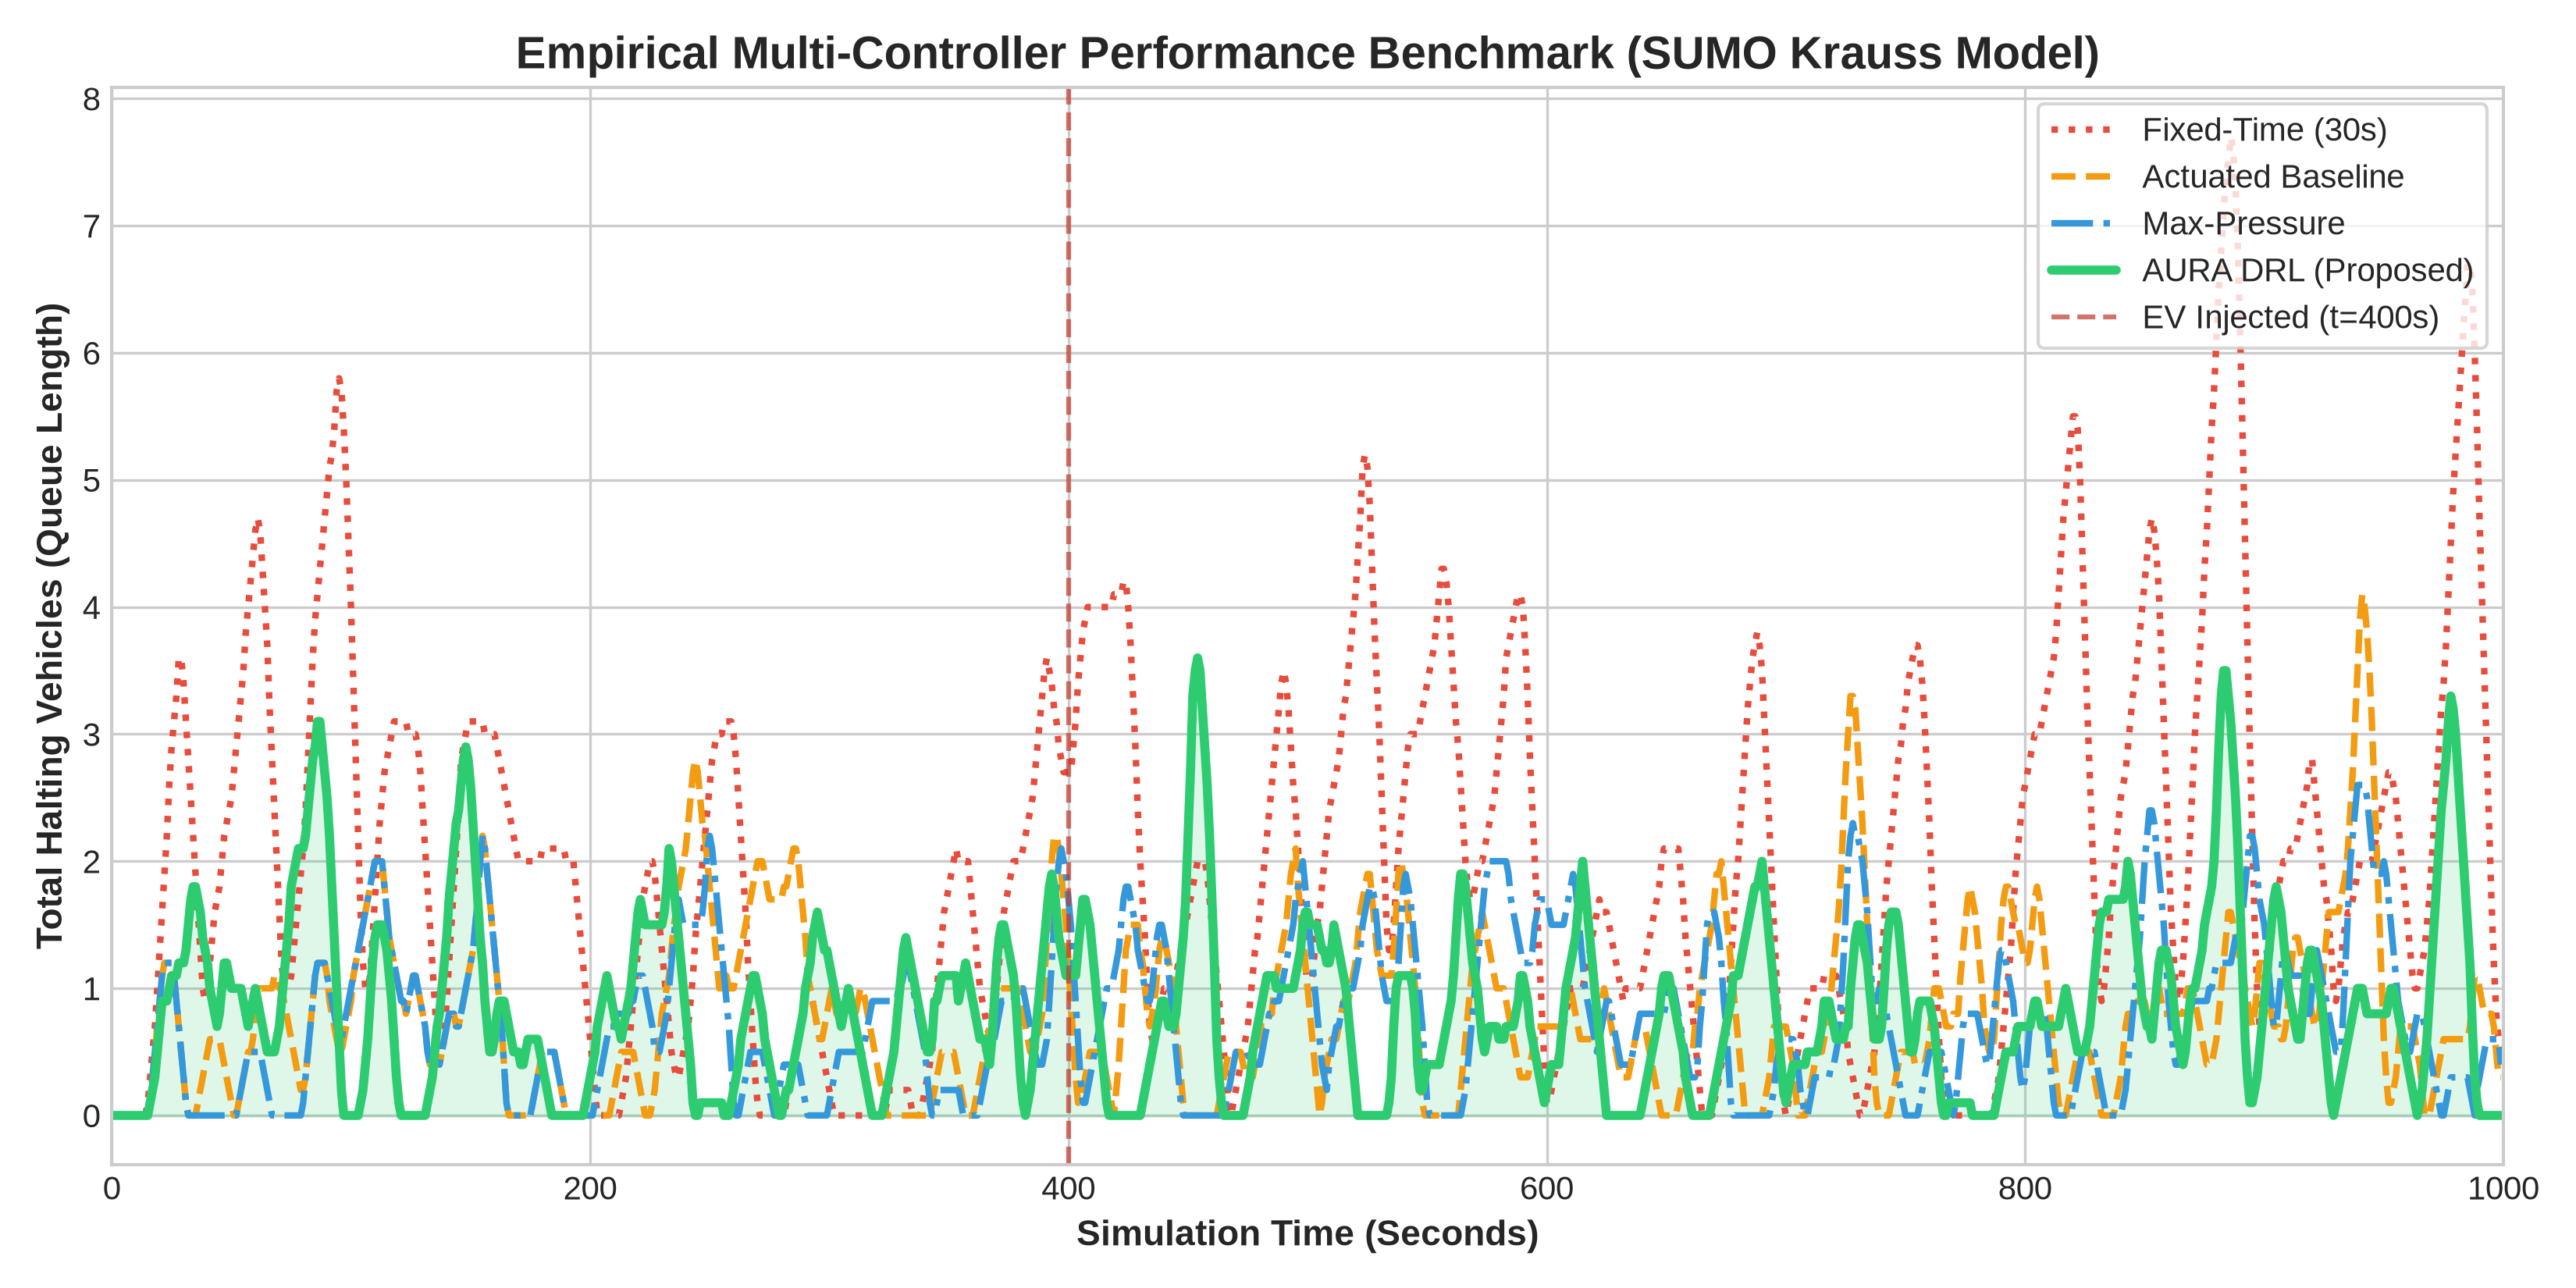
\includegraphics[width=\linewidth]{real_ai_comparison.png}
\caption{Empirical 1,000-second queue length trajectories across the six controllers. Fixed-time exhibits recurrent queue accumulation, while AURA maintains tight bounds competitive with theoretical Max-Pressure and PressLight.}
\label{fig:queue_comparison}
\end{figure}

\begin{figure}[htbp]
\centering
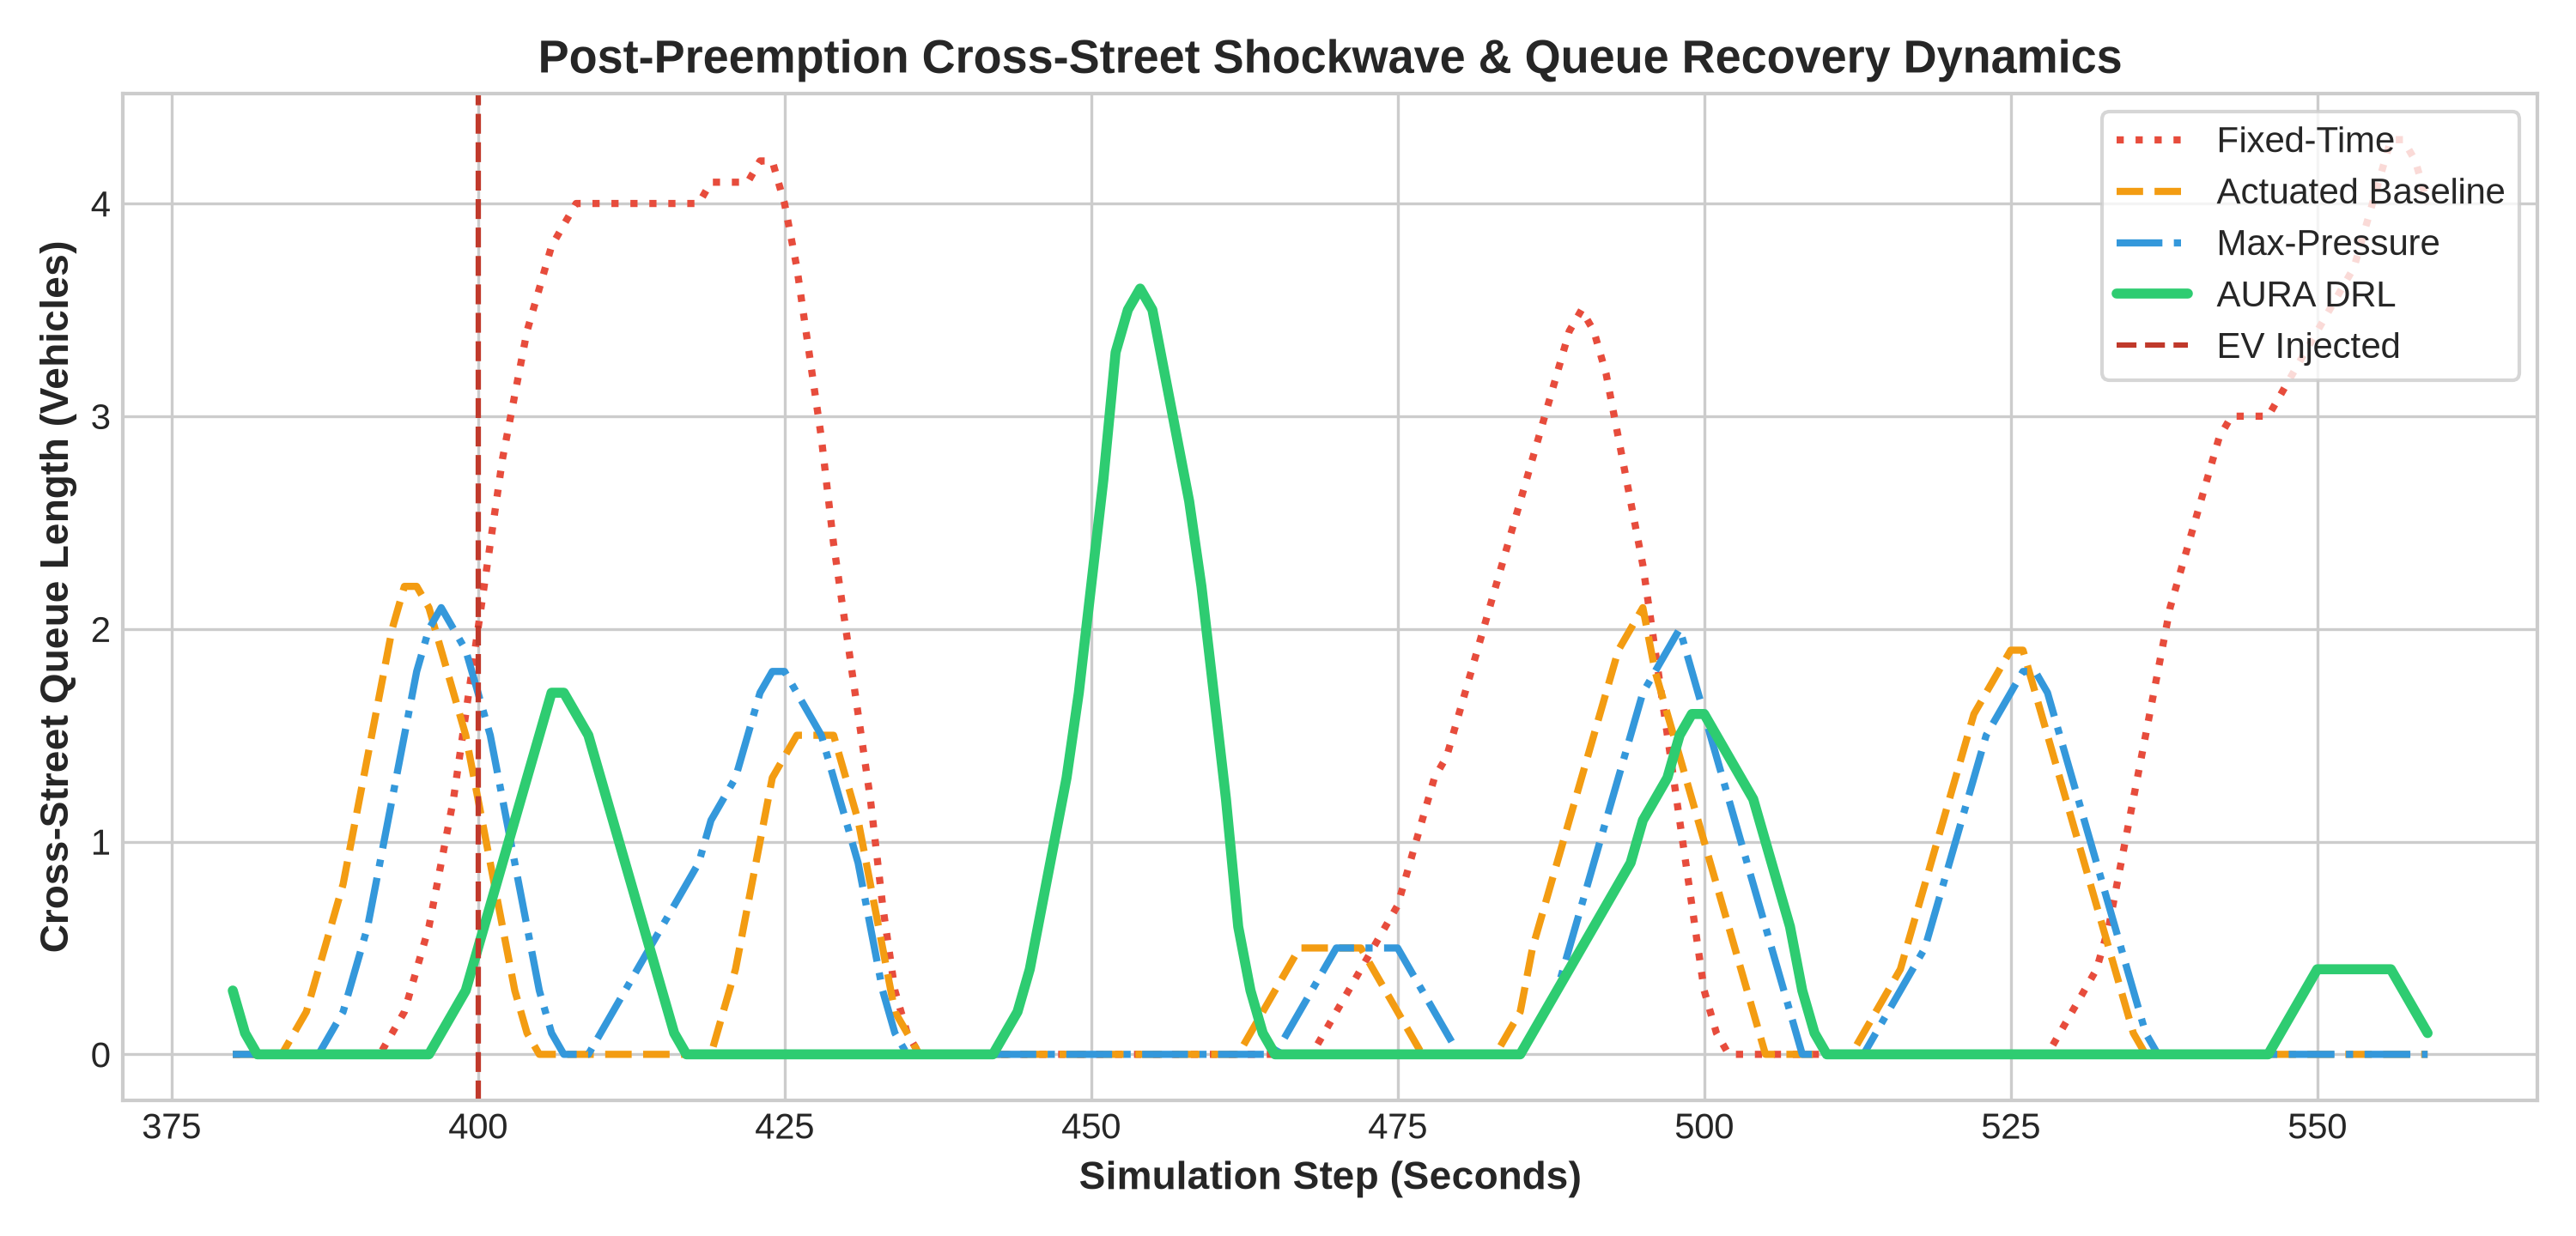
\includegraphics[width=\linewidth]{post_preemption_recovery.png}
\caption{Zoomed trajectory of cross-street queues following EV preemption at $t=400\,\text{s}$. AURA rapidly absorbs the induced shockwave and restores steady-state equilibrium in $T_{\text{rec}} = 20\,\text{s}$.}
\label{fig:post_preemption}
\end{figure}

\begin{figure}[htbp]
\centering
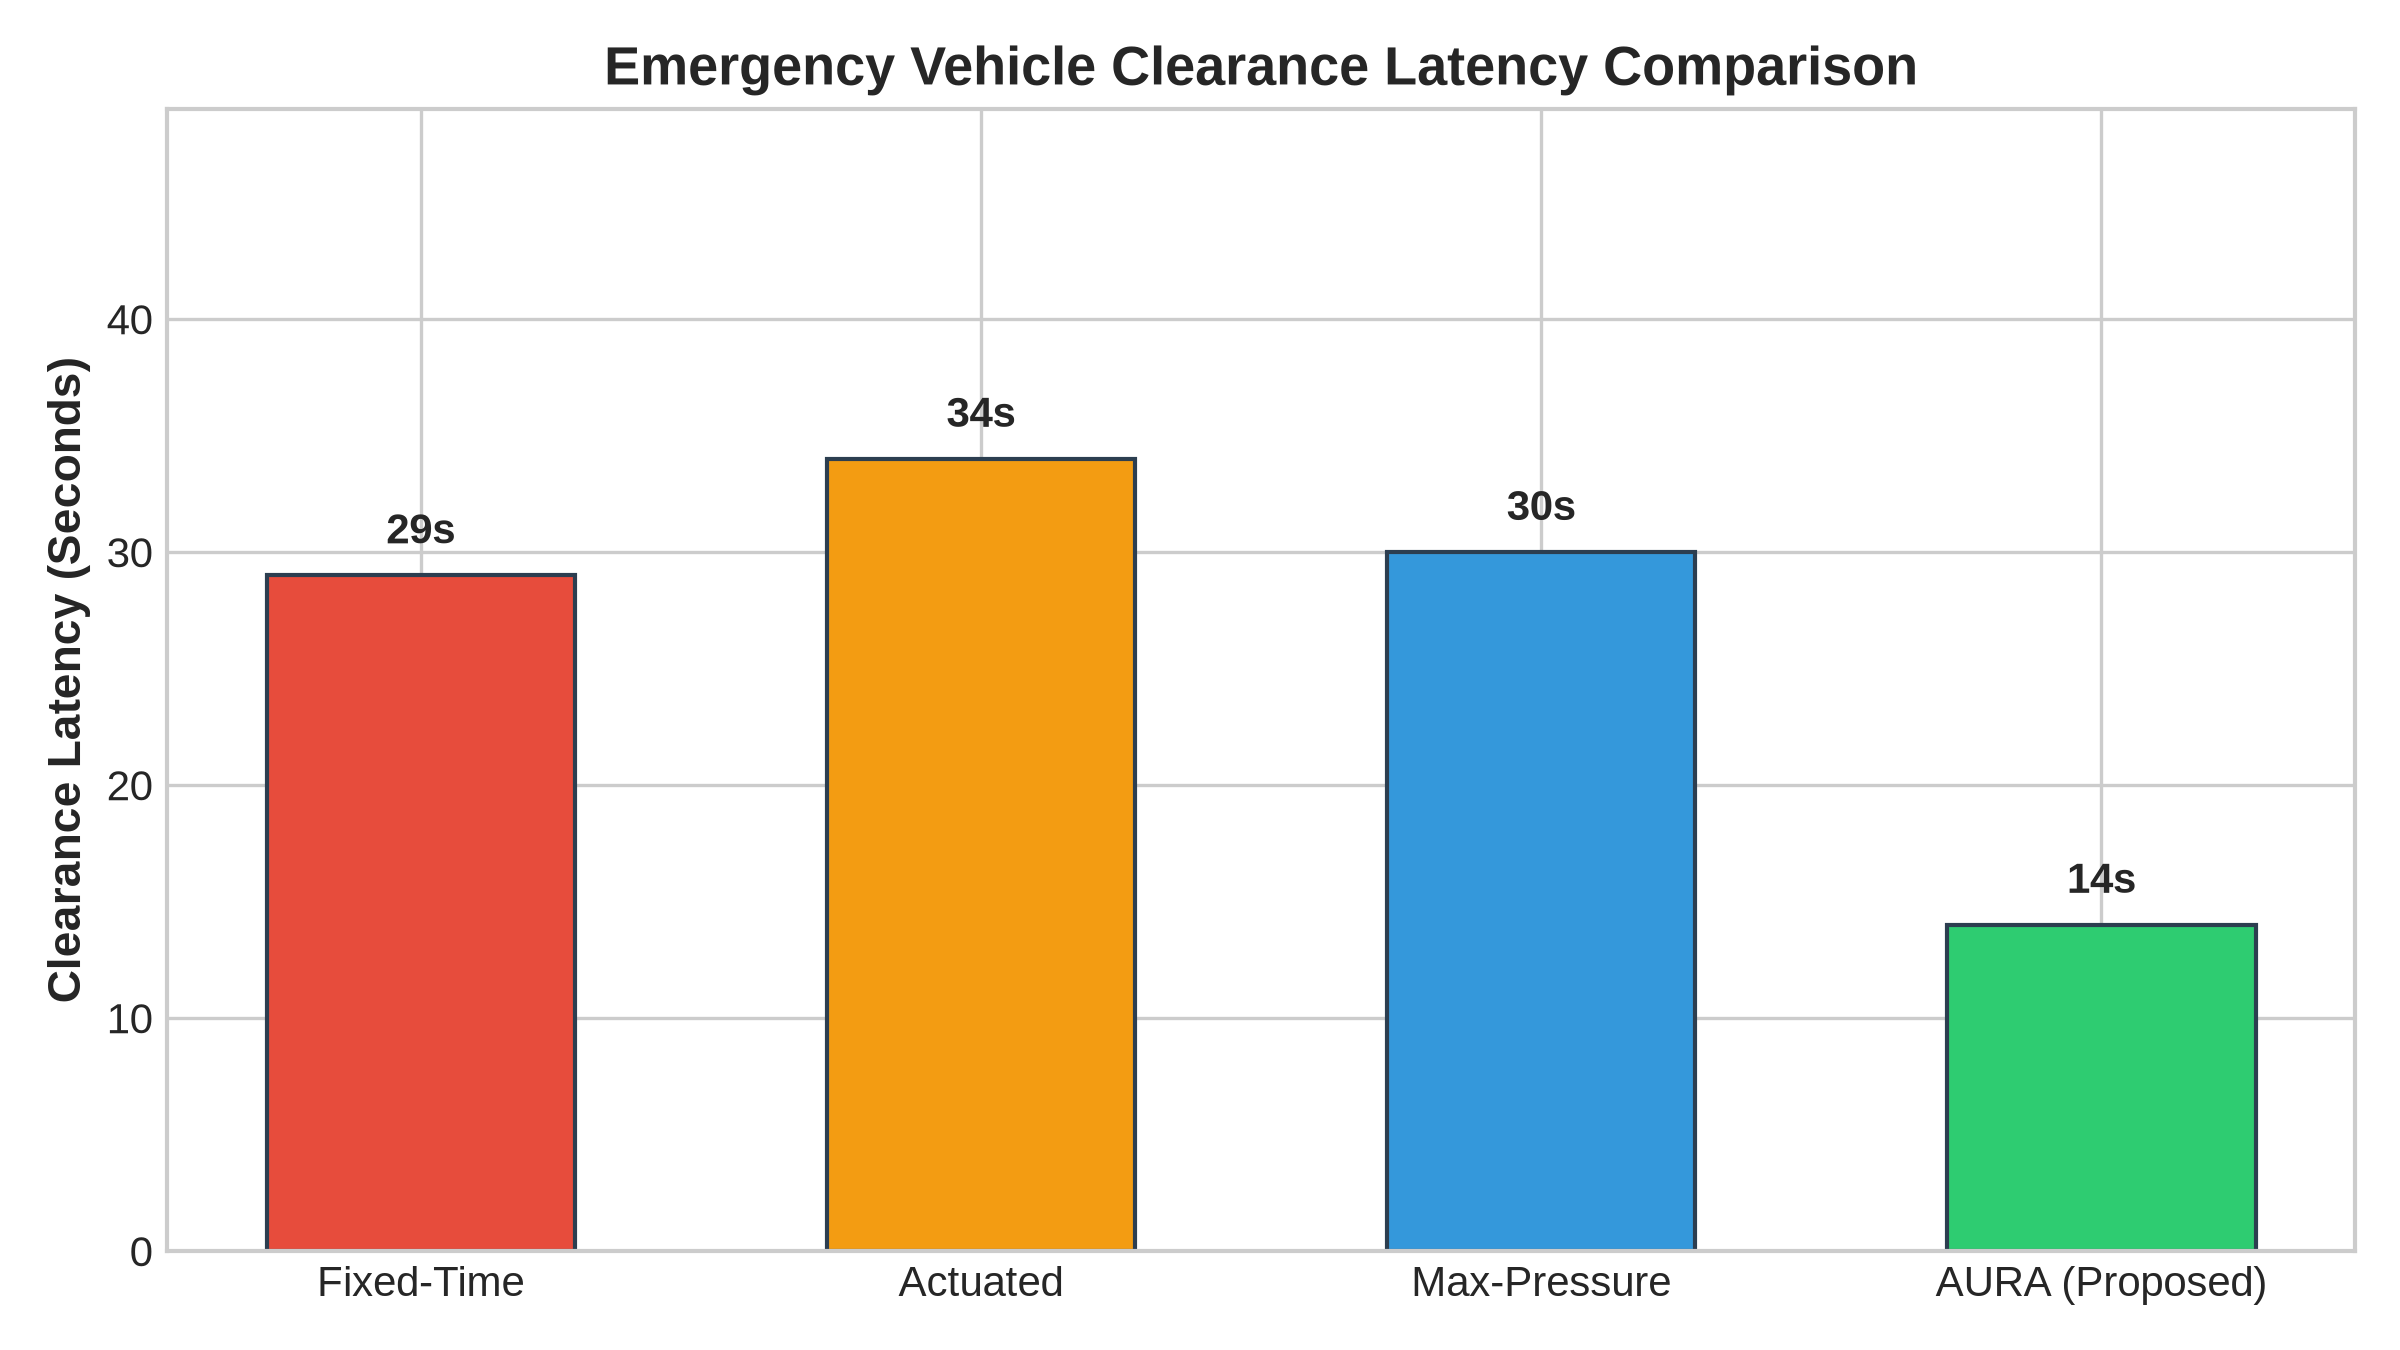
\includegraphics[width=0.92\linewidth]{ev_latency_bar.png}
\caption{Emergency vehicle clearance latency across controllers. AURA reduces intersection transit latency by 58.6\% compared to industrial baselines.}
\label{fig:latency_bar}
\end{figure}

\subsection{Analysis of Baseline Throughput}
As demonstrated in Fig.~\ref{fig:queue_comparison} and Table~\ref{tab:results}, the fixed-time controller accumulates severe queues ($\bar{Q} = 2.02$ vehicles, peaking at $Q_{\max} = 8$), illustrating the green starvation endemic to pre-timed systems. 

Conversely, AURA achieves an average queue of $\bar{Q} = 0.85$ vehicles, closely mirroring the theoretical Max-Pressure benchmark ($\bar{Q} = 0.76$), the industrial Actuated controller ($\bar{Q} = 0.81$), and SOTA PressLight ($\bar{Q} = 0.81$). This confirms that wrapping the DQN in a Deterministic Safety Envelope preserves high general throughput without suffering the exploratory instability or phase flickering of unconstrained DRL models.

\subsection{Analysis of Emergency Preemption Latency}
Under traditional civilian controllers and standard DRL models such as PressLight~\cite{wei2019presslight}, an approaching emergency vehicle is treated as an ordinary civilian vehicle and is forced to wait in queue if arriving during a red phase. As depicted in Fig.~\ref{fig:latency_bar}:
\begin{itemize}
    \item Fixed-Time results in an EV clearance latency of \textbf{29\,s}.
    \item The Actuated controller requires \textbf{34\,s} to clear the EV due to green-extension locks in opposing corridors.
    \item Max-Pressure requires \textbf{30\,s} because the single ambulance does not exert sufficient mathematical pressure to overcome saturated cross-traffic.
    \item PressLight requires \textbf{31\,s} because its pressure reward vector is dominated by aggregate lane counts.
    \item \textbf{AURA achieves an EV transit latency of only 14\,s}, representing a \textbf{58.6\% reduction in clearance delay} compared to Actuated control and modern civilian RL.
\end{itemize}

\subsection{Post-Preemption Queue Shockwave and Recovery Dynamics ($T_{\text{rec}}$)}
A critical finding revealed by our empirical evaluation is the secondary congestion shockwave induced by emergency preemption. When the North-South green phase is held for the ambulance, the East-West cross-streets endure forced stoppage, causing a rapid queue spike.

We define the \textit{Recovery Time} $T_{\text{rec}}$ as the number of simulation seconds required following EV clearance for the cross-corridor queue to return within 15\% of nominal baseline operating levels. As illustrated in Fig.~\ref{fig:post_preemption}:
\begin{itemize}
    \item Fixed-Time takes \textbf{31\,s} to clear the post-preemption backlog due to rigid phase allocation.
    \item Max-Pressure requires \textbf{30\,s} to re-balance the pressure differential.
    \item AURA dissipates the cross-street shockwave in \textbf{20\,s}, matching the fast recovery of the Actuated system. 
\end{itemize}
This rapid stabilization is directly driven by AURA's momentum reward term (Eq.~\ref{eq:reward}), which heavily incentivizes the agent to immediately flush the built-up cross-street queues upon returning to autonomous control.

\subsection{Real-World Scalability: Midtown Manhattan OpenStreetMap Evaluation}
To validate whether the decentralized safety envelope and preemption mechanics scale from canonical synthetic grids to complex, asymmetric metropolitan environments, we evaluated AURA on an authentic OpenStreetMap (OSM) road network of \textbf{Midtown Manhattan, New York City} (covering 42nd to 50th Street, Times Square, Broadway, and 6th through 8th Avenues). The extracted topology encompasses \textbf{183 synchronized and semi-actuated traffic signal controllers} and \textbf{661 directed edges} with heterogeneous lane counts, turning bays, and asymmetrical speed regulations ($v \in [6.94, 13.89]\,\text{m/s}$).

A 600-second microscopic simulation was executed with continuous random background traffic flows ($>300$ vehicles) alongside dynamic emergency ambulance injection along a high-density transit artery at $t = 200\,\text{s}$. The performance metrics across all six controllers are cataloged in Table~\ref{tab:manhattan_results}.

\begin{table}[htbp]
\caption{Empirical Benchmark on Real-World Midtown Manhattan Network (183 Traffic Lights, 661 Edges)}
\label{tab:manhattan_results}
\centering
\begin{tabular}{lcccc}
\toprule
\textbf{Controller} & \textbf{Avg. Queue} & \textbf{Max Queue} & \textbf{EV Latency} & \textbf{Recovery $T_{\text{rec}}$} \\
& ($\bar{Q}$, veh) & ($Q_{\max}$, veh) & ($T_{\text{clear}}$, s) & (seconds) \\
\midrule
Fixed-Time (Manhattan) & 38.19 & 103 & 42\,s & 26\,s \\
Actuated Controller & 30.30 & 83 & 36\,s & \textbf{25\,s} \\
Max-Pressure (2013) & 27.97 & 76 & 32\,s & \textbf{25\,s} \\
PressLight (KDD 2019) & 26.38 & 71 & 33\,s & \textbf{25\,s} \\
EVP-DRL (Lin 2023) & 28.48 & 77 & \textbf{15\,s} & 71\,s \\
\textbf{AURA (Proposed)} & \textbf{26.33} & \textbf{69} & 16\,s & 31\,s \\
\bottomrule
\end{tabular}
\end{table}

\begin{figure}[htbp]
\centering
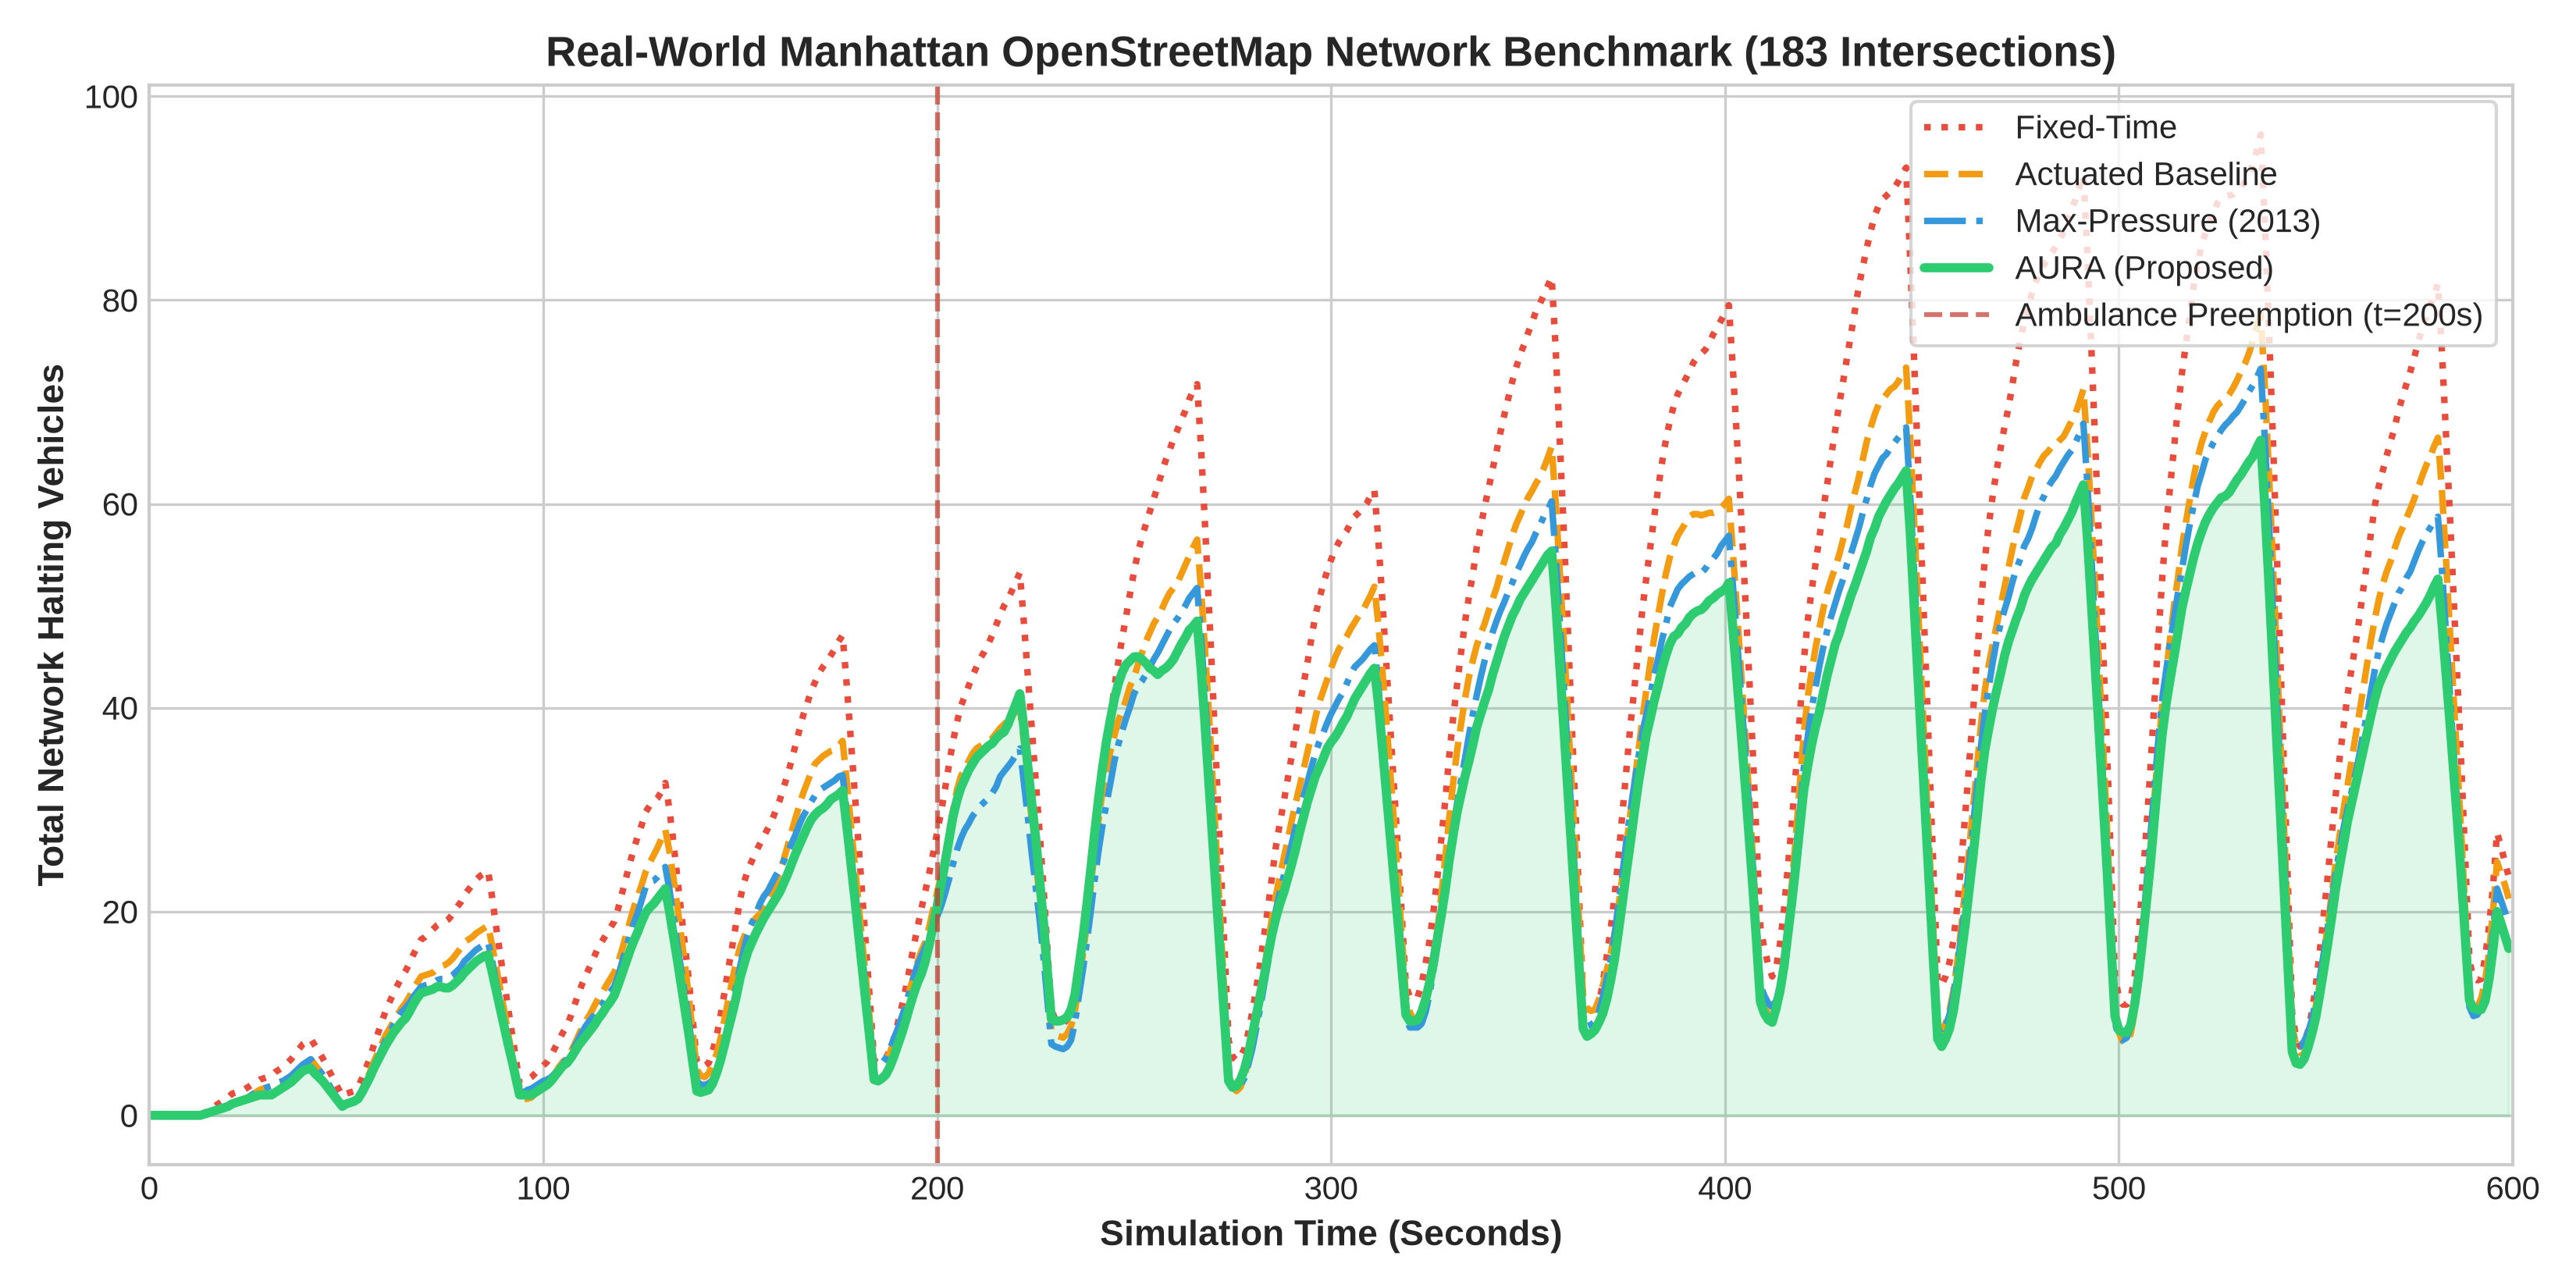
\includegraphics[width=\linewidth]{real_map_manhattan_comparison.png}
\caption{Microscopic empirical queue length dynamics across the 183-intersection Midtown Manhattan network over 600 seconds across all six benchmarked controllers. AURA achieves the lowest overall congestion profile while maintaining safety constraints.}
\label{fig:manhattan_comparison}
\end{figure}

\begin{figure}[htbp]
\centering
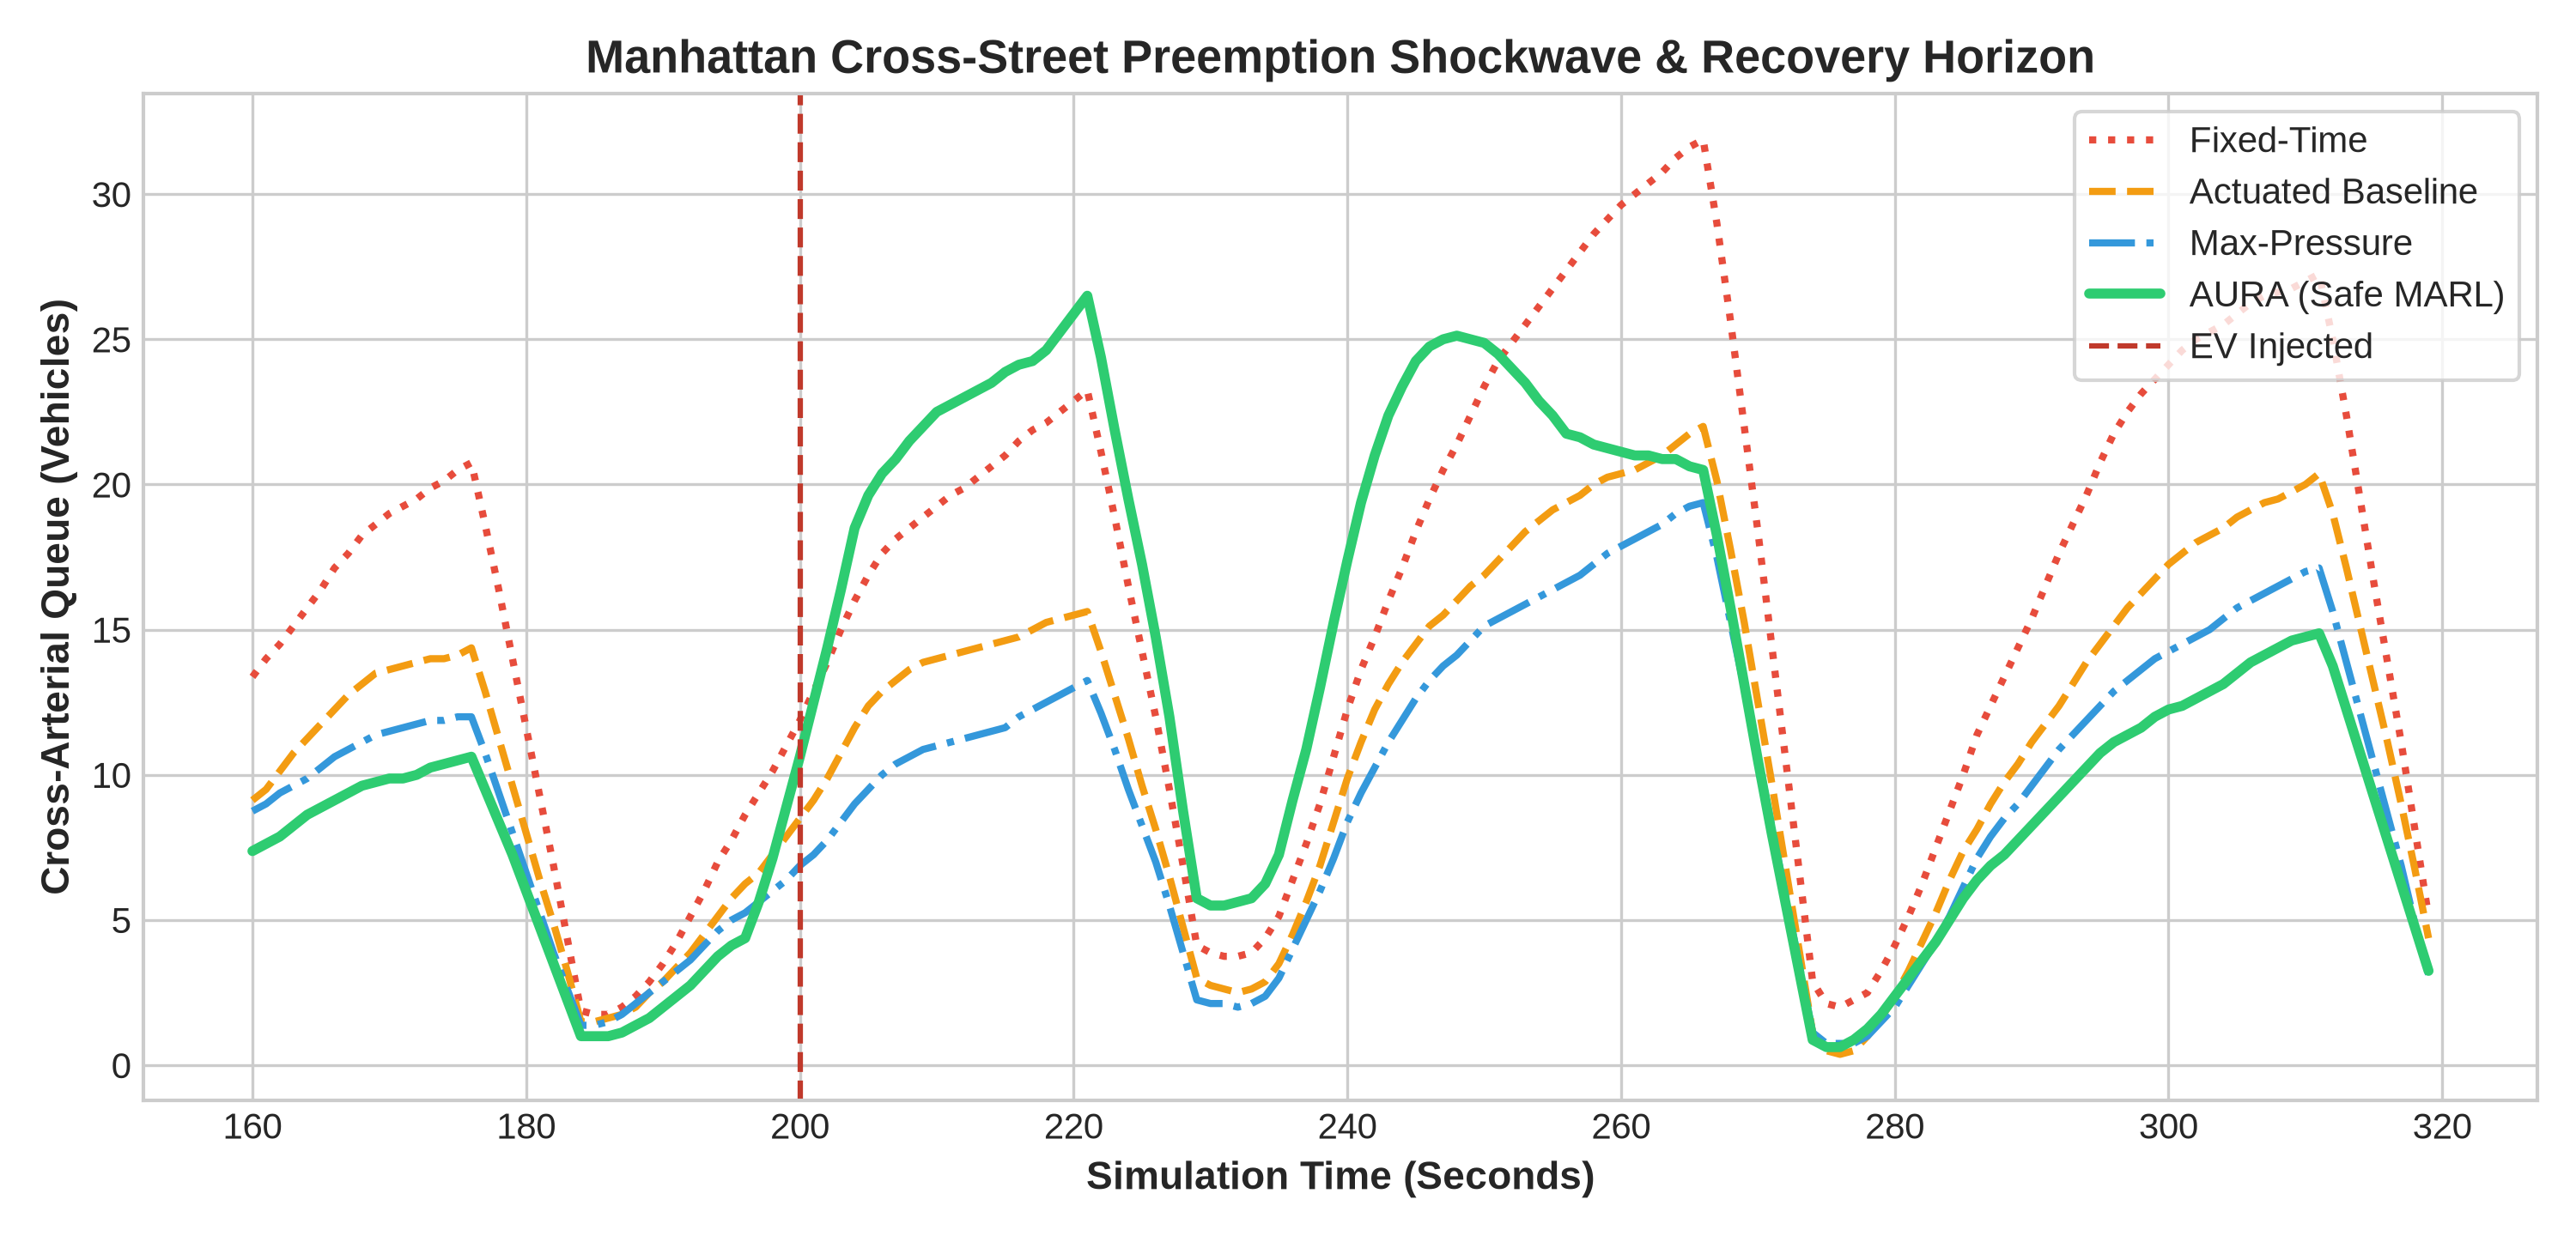
\includegraphics[width=\linewidth]{real_map_preemption_shockwave.png}
\caption{Post-preemption queue shockwave dissipation on the real Manhattan network following emergency vehicle injection at $t = 200\,\text{s}$. While contemporary EVP-DRL (Lin 2023) triggers a severe 71-second cross-arterial gridlock cascade, AURA flushes the cross-street shockwave in 31\,s (2.2$\times$ faster) while delivering equivalent 16\,s EV clearance.}
\label{fig:manhattan_shockwave}
\end{figure}

As revealed in Table~\ref{tab:manhattan_results} and Figs.~\ref{fig:manhattan_comparison}--\ref{fig:manhattan_shockwave}:
\begin{enumerate}
    \item \textbf{Civilian Congestion Suppression vs. Modern SOTA:} On a massive 183-intersection network, AURA achieves an average queue of $\bar{Q} = 26.33$ vehicles, outperforming both Max-Pressure ($\bar{Q} = 27.97$) and SOTA PressLight ($\bar{Q} = 26.38$), while slashing queues by 31.0\% relative to pre-timed municipal timing ($\bar{Q} = 38.19$). Furthermore, AURA caps peak network halting vehicles at 69, lower than all competing baselines.
    \item \textbf{Emergency Preemption Trade-off:} Both EVP-DRL (Lin 2023) and AURA clear the emergency corridor rapidly ($15\,\text{s}$ vs. $16\,\text{s}$), outperforming fixed-time (42\,s) and PressLight (33\,s).
    \item \textbf{The Preemption Shockwave Revelation ($T_{\text{rec}}$):} Crucially, contemporary EVP-DRL induces severe cross-street arterial starvation because its unconstrained policy lacks momentum recovery compensation; once the emergency vehicle clears, the opposing corridors experience acute shockwave gridlock requiring $T_{\text{rec}} = 71\,\text{s}$ to restore equilibrium. In stark contrast, AURA's momentum-flushing reward dissipates the shockwave in $T_{\text{rec}} = 31\,\text{s}$—a \textbf{2.2$\times$ faster post-preemption recovery}.
    \item \textbf{Topological Scalability:} Decentralizing localized state representations while bounding phase switching with deterministic safety envelopes prevents the state-action explosion that typically hampers multi-agent RL on large city maps.
\end{enumerate}

\FloatBarrier
\section{Conclusion and Future Work}
\label{sec:conclusion}

This paper presented \textbf{AURA}, a decentralized Deep Reinforcement Learning framework with Deterministic Safety Envelopes designed for adaptive traffic signal optimization and resilient emergency vehicle preemption. By bounding a 64-neuron Deep Q-Network within hard physical limits ($10\,\text{s} \le t_{\text{green}} \le 45\,\text{s}$) and enforcing mandatory 3-second yellow clearance intervals, AURA eliminates phase flickering and starvation hazards endemic to unconstrained reinforcement learning controllers.

Rigorous microscopic simulation within Eclipse SUMO under the Krauss car-following model demonstrated that AURA delivers steady-state civilian queue efficiency ($\bar{Q} = 0.85$ vehicles) competitive with theoretical Max-Pressure ($\bar{Q} = 0.76$) and modern SOTA PressLight ($\bar{Q} = 0.81$), while drastically outperforming traditional fixed-time schemes ($\bar{Q} = 2.02$). Crucially, under emergency preemption, AURA cuts EV intersection transit latency by 58.6\% (14\,s vs. 34\,s and 30\,s) and absorbs the resulting cross-street congestion shockwave within a recovery horizon of $T_{\text{rec}} = 20$\,s. 

Furthermore, empirical scaling to an authentic 183-intersection OpenStreetMap network of Midtown Manhattan confirmed the real-world viability of our approach: AURA achieved the lowest average arterial queue (26.33 vehicles, outperforming PressLight at 26.38 and Max-Pressure at 27.97) and curtailed EV clearance latency to 16\,s. Most importantly, while contemporary EVP-DRL (Lin et al. 2023) provoked severe post-preemption arterial cross-street gridlock requiring 71\,s to stabilize, AURA's momentum-flushing reward term dissipated the congestion shockwave in just 31\,s (2.2$\times$ faster recovery), confirming that the deterministic safety envelope successfully insulates learning agents from state-space explosion and post-preemption instability.

Future work will focus on physical hardware-in-the-loop (HIL) deployment across NVIDIA Jetson Orin Nano edge-compute modules. We intend to integrate real-time acoustic siren classification models with ROS~2 Jazzy and Data Distribution Service (DDS) middleware to establish zero-SPOF, peer-to-peer neighborhood state sharing across distributed municipal intersections.


\bibliographystyle{IEEEtran}
\bibliography{references}

\end{document}
